%%
%% Automatically generated ptex2tex (extended LaTeX) file
%% from Doconce source
%% http://code.google.com/p/doconce/
%%




%-------------------------- begin preamble --------------------------
\documentclass[twoside]{article}



\usepackage{relsize,epsfig,makeidx,amsmath,amsfonts,graphicx,caption,subcaption,fullpage}
\usepackage[latin1]{inputenc}
%\usepackage{minted} % packages needed for verbatim environments


% Hyperlinks in PDF:
\usepackage[%
    colorlinks=true,
    linkcolor=black,
    %linkcolor=blue,
    citecolor=black,
    filecolor=black,
    %filecolor=blue,
    urlcolor=black,
    pdfmenubar=true,
    pdftoolbar=true,
    urlcolor=black,
    %urlcolor=blue,
    bookmarksdepth=3   % Uncomment (and tweak) for PDF bookmarks with more levels than the TOC
            ]{hyperref}
%\hyperbaseurl{}   % hyperlinks are relative to this root

% Tricks for having figures close to where they are defined:
% 1. define less restrictive rules for where to put figures
\setcounter{topnumber}{2}
\setcounter{bottomnumber}{2}
\setcounter{totalnumber}{4}
\renewcommand{\topfraction}{0.85}
\renewcommand{\bottomfraction}{0.85}
\renewcommand{\textfraction}{0.15}
\renewcommand{\floatpagefraction}{0.7}
% 2. ensure all figures are flushed before next section
\usepackage[section]{placeins}
% 3. enable begin{figure}[H] (often leads to ugly pagebreaks)
%\usepackage{float}\restylefloat{figure}
\usepackage{parskip}

\newcommand{\inlinecomment}[2]{  ({\bf #1}: \emph{#2})  }
%\newcommand{\inlinecomment}[2]{}  % turn off inline comments
\newcommand{\dutt}{\frac{\partial^2 u}{\partial t^2}}
\newcommand{\duxx}{\frac{\partial^2 u}{\partial x^2}}
\newcommand{\dut}{\frac{\partial u}{\partial t}}
\newcommand{\dux}{\frac{\partial u}{\partial x}}
\newcommand{\dtt}{\Delta t^2}
\newcommand{\dxx}{\Delta x^2}
\newcommand{\dt}{\Delta t}
\newcommand{\dx}{\Delta x}
\newcommand{\wt}{\tilde{\omega}}

% insert custom LaTeX commands...

\makeindex

\begin{document}
%-------------------------- end preamble --------------------------





% ----------------- title -------------------------

\begin{center}
{\LARGE\bf INF5620 Second Project}\\
{\LARGE\bf Wave Equation - Finte elements}
\end{center}




% ----------------- author(s) -------------------------

\begin{center}
{\bf Nina Kristine Kylstad (\texttt{ninakky@student.matnat.uio.no})} \\ [0mm]
\end{center}

\vspace{0.5cm}
\begin{center}
% List of all institutions:
\centerline{INF5620 - Numerical methods for partial differential equations}
\end{center}
% ----------------- end author(s) -------------------------



% ----------------- date -------------------------


\begin{center}
November 08, 2012
\end{center}

\vspace{1cm}


\begin{abstract}
This report investigates the one dimensional wave equation,
and using finite element methods for solving a wave equation.
\end{abstract}

\tableofcontents



% Section with multi-line equation.


\section{Mathematical problem}

\label{math:problem}

\index{model problem} \index{1D wave equation}

We consider the initial- and boundary-value problem given by 
\begin{align}
\dutt &= c^2 \duxx,	\label{1D:wave:eq}\\
u(0,t) &= U_0(t),  	\label{bc:x0}\\
\dux(L) &= 0, 		\label{bc:dux:xL}\\
u(x,0) &= I(x),		\label{ic:t0}\\
\dut(x,0) &= V(x),	\label{ic:dut:t0}
\end{align}

where \eqref{1D:wave:eq} is the 1D wave equation, \eqref{bc:x0} and \eqref{bc:dux:xL} are boundary condition and \eqref{ic:t0} and \eqref{ic:dut:t0} are initial conditions. 

\section{Numerical solution}

\subsection{Finite differences}
\label{finite:differences}

We use finite differences to discretize the equation in time. We use a centered difference to approximate the time derivative:
\begin{equation*}
\dutt \approx \frac{u^{n+1} - 2u^n + u^{n-1}}{\Delta t^2}
\end{equation*}

This gives (in compact form):
\begin{equation}
\left[D_tD_tu  = c^2u_{xx}\right]^n
\end{equation}

Expanded and rearranged, this gives the scheme

\begin{equation}
u^{n+1} = 2u^n - u^{n-1} + \Delta t^2 c^2 u^n_{xx}
\end{equation}

We then use the following approximations for $u(x):$
\begin{align}
u^n(x) &\approx \sum^N_{j=0} c_j^n\phi_j(x),     \label{u:n:approx}\\
u^{n-1}(x) &\approx \sum^N_{j=0} c_j^{n-1}\phi_j(x),     \label{u:n-1:approx}\\
u^{n+1}(x) &\approx \sum^N_{j=0} c_j^{n+1}\phi_j(x),     \label{u:n+1:approx}
\end{align}


\subsection{Using a Galerkin method to derive variational form}

We continue by using a Galerkin method with $v(x)$ as a test function, in order to obtain variational form:

\begin{equation}
\int\limits^L_0 u^{n+1} v dx = \int\limits^L_0 2u^{n} v dx + \int\limits^L_0 -u^{n-1} v dx + \int\limits^L_0 
\Delta t^2c^2 u^n_{xx} v dx
\label{galerkin:start}
\end{equation}

We use integration by parts for the final term:

\begin{align*}
\int\limits^L_0 \Delta t^2c^2 u^n_{xx} v dx &= -\Delta t^2c^2 \int\limits^L_0 u^n_x v_x dx + 
\Delta t^2c^2 \left[u_x^n v\right]^L_0 \\
\left[u_x^n v\right]^L_0 &= u_x^n(L) v(L) - u_x^n(0) v(0) = 0
\end{align*}
This result comes from using the boundary conditions \eqref{bc:x0} and \eqref{bc:dux:xL}. Inserting this back into \eqref{galerkin:start} gives

\begin{equation}
\int\limits^L_0 u^{n+1} v dx = 2\int\limits^L_0 u^{n} v dx - \int\limits^L_0 u^{n-1} v dx - 
\Delta t^2c^2 \int\limits^L_0 u^n_x v_x dx
\label{var:form:one}
\end{equation} 


\subsection{Deriving a linear system}


We now replace the $u$-terms in \eqref{var:form:one} with the approximations \eqref{u:n:approx}, \eqref{u:n-1:approx} and \eqref{u:n+1:approx}. We also replace the test function $v$ with $v = \phi_i(x)$. This gives

\begin{align}
\sum^N_{j=0}\left(\int\limits_0^L \phi_i \phi_j dx\right) c_j^{n+1} &=
2 \sum^N_{j=0}\left(\int\limits_0^L \phi_i \phi_j dx\right) c_j^{n} - 
\sum^N_{j=0}\left(\int\limits_0^L \phi_i \phi_j dx\right) c_j^{n-1} - 
\Delta t^2c^2 \sum^N_{j=0}\left(\int\limits_0^L \phi_i' \phi_j' dx\right) c_j^{n}
\end{align}

This gives the linear system

\begin{equation}
\mathbf{Mc^{n+1}} = 2\mathbf{Mc^{n}} - \mathbf{Mc^{n-1}} - C^2\mathbf{Kc^{n}}
\end{equation}

where $C = \Delta t c$.


\subsection{Interpreting as finite differences}

We begin by looking at the matrices $M$ and $K$. The entries in $M$ are given by $M_{i,j} = \int\limits_0^L\phi_i\phi_j$, and the entries in $K$ are given by $K_{i,j} = \int\limits_0^L\phi_i'\phi_j'$. Using P1 elements, we get the matrices
\begin{equation}
M = \frac{h}{6}\left[
\begin{matrix}
2 & 1 & 0 & \hdots & 0\\
1 & 4 & 1 & \ddots & \vdots\\
0 & \ddots & \ddots & \ddots & 0\\
\vdots & \ddots & 1 & 4 & 1\\
0 & \hdots & 0 & 1 & 2\\
\end{matrix}\right] 
\end{equation}

and

\begin{equation}
K = \frac{1}{h}\left[
\begin{matrix}
2 & -1 & 0 & \hdots & 0\\
-1 & 2 & -1 & \ddots & \vdots\\
0 & \ddots & \ddots & \ddots & 0\\
\vdots & \ddots & -1 & 2 & -1\\
0 & \hdots & 0 & -1 & 2\\
\end{matrix}\right] 
\end{equation}

We now look at equation number $i$ in the linear system, which becomes

\begin{align*}
\frac{h}{6}c_{i-1}^{n+1} + \frac{4h}{6}c_{i}^{n+1} + \frac{h}{6}c_{i+1}^{n+1} = &2\left(\frac{h}{6}c_{i-1}^{n} + \frac{4h}{6}c_{i}^{n} + \frac{h}{6}c_{i+1}^{n}\right)\\
&- \left(\frac{h}{6}c_{i-1}^{n-1} + \frac{4h}{6}c_{i}^{n-1} +\frac{h}{6}c_{i+1}^{n-1}\right)\\
&- C^2\left( \frac{-1}{h}c_{i-1}^{n} + \frac{2}{h}c_{i}^{n} + \frac{-1}{h}c_{i+1}^{n}\right)
\end{align*}

We can replace $c_i^n$ with $u_i^n$ because the coefficients $c_i$ are the values of $u$ at spacial point $i$. $h$ is the space between the nodes, also known as $\Delta x$. This gives

\begin{align*}
\frac{1}{6}u_{i-1}^{n+1} + \frac{4}{6}u_{i}^{n+1} + \frac{1}{6}u_{i+1}^{n+1} = &\frac{2}{6}u_{i-1}^{n} + \frac{8}{6}u_{i}^{n} + \frac{2}{6}u_{i+1}^{n}\\
&- \frac{1}{6}u_{i-1}^{n-1} - \frac{4}{6}u_{i}^{n-1} -\frac{1}{6}u_{i+1}^{n-1}\\
&+ \frac{\Delta t^2 c^2}{\Delta x^2}\left(u_{i-1}^{n} -2u_{i}^{n} + u_{i+1}^{n}\right)
\end{align*}

We move some terms around, and get
\begin{align*}
&\frac{u_{i}^{n+1} - 2u_{i}^{n} + u_{i}^{n-1}}{\Delta t^2} + 
\frac{1}{6\Delta t^2}\left(u_{i-1}^{n+1} -2 u_{i}^{n+1} + u_{i+1}^{n+1} - 2u_{i-1}^{n} + 4u_{i}^{n} - 2u_{i+1}^{n} + u_{i-1}^{n-1}
-2u_{i}^{n-1} +  u_{i+1}^{n-1}\right)\\
 &= c^2\frac{u_{i-1}^{n} -2u_{i}^{n} + u_{i+1}^{n}}{\Delta x^2}
\end{align*}

We see that the first term is the finite difference (FD) approximation for the 2nd derivative of $u$ in time, $[D_tD_t u]^n_i$, and the last term is the FD approximation for the 2nd derivative of $u$ in space, $[D_xD_x u]_i^n$. The term in the middle is a combination of the two, and can be written as $[D_tD_t(\frac{1}{6}\Delta x^2 D_xD_x u)]_i^n$. (Note: We have to multiply by $\Delta x^2$ in the middle term to be able to write it as the approximation to the 2nd derivative in space.)

Combining the three terms, we get,

\begin{equation}
[D_tD_t(u + \frac{1}{6}\Delta x^2 D_xD_x u) = c^2D_xD_x u]^n_i  
\label{FD:scheme}
\end{equation}


\subsection{Analysing the scheme in \eqref{FD:scheme}}

To perform an analysis of the scheme \eqref{FD:scheme}, we introduce a Fourier component, $u = e^{i(kx-\tilde{\omega}t)}$

We then get 

\begin{align*}
[D_tD_t u]^n_p &= -\frac{4}{\dtt}sin^2\left(\frac{\tilde{\omega}\dt}{2}\right)e^{-i\tilde{\omega}n\dt}e^{ikp\dx}, \\
[D_xD_x u]^n_p &= -\frac{4}{\dxx}sin^2\left(\frac{k\dx}{2}\right) e^{-i\tilde{\omega}n\dt}e^{ikp\dx}, \\
[D_tD_t(\frac{1}{6}\dxx D_xD_x u)]^n_p &= \frac{1}{6}\dxx[D_tD_te^{-i\tilde{\omega}t}]^n[D_xD_xe^{ikx}]_p\\
&= \frac{8}{3\dtt}e^{-i\tilde{\omega}n\dt}e^{ikp\dx}sin^2\left(\frac{\tilde{\omega}\dt}{2}\right)sin^2\left(\frac{k\dx}{2}\right)
\end{align*}

Putting this into the scheme \eqref{FD:scheme}, we get

\begin{align*}
&-\frac{4}{\dtt}sin^2\left(\frac{\tilde{\omega}\dt}{2}\right)e^{-i\tilde{\omega}n\dt}e^{ikp\dx} + \frac{8}{3\dtt}e^{-i\tilde{\omega}n\dt}e^{ikp\dx}sin^2\left(\frac{\tilde{\omega}\dt}{2}\right)sin^2\left(\frac{k\dx}{2}\right)\\
&= -\frac{4}{\dxx}sin^2\left(\frac{k\dx}{2}\right) e^{-i\tilde{\omega}n\dt}e^{ikp\dx}
\end{align*}

After some simplification, we are left with

\begin{align}
sin^2\left(\frac{\tilde{\omega}\dt}{2}\right) &= C^2 \frac{sin^2\left(\frac{k\dx}{2}\right)}{1 - \frac{2}{3}sin^2\left(\frac{k\dx}{2}\right)}\nonumber\\
sin\left(\frac{\tilde{\omega}\dt}{2}\right) &= C \frac{sin\left(\frac{k\dx}{2}\right)}{\sqrt{1 - \frac{2}{3}sin^2\left(\frac{k\dx}{2}\right)}} \label{sin:omega}
\end{align}

Since $\omega$ is real, we are also looking for a real $\tilde{\omega}$. This means that the left-hand-side of \eqref{sin:omega} must be in the interval $[-1,1]$, and therefore som must the right-hand-side. The $sin$ part of the right-hand-side only varies between $-1$ and $1$. We therefore choose one of the extremes to find a stability limit for $C$. We choose $sin(k\dx/2) = 1$, which means that the left-hand-side must be smaller than, or equal to, $1$ (the upper boundary of the left-hand-side).

\begin{align*}
C\frac{1}{1 - \frac{2}{3}} &\leq 1\\
C & \leq \sqrt{1 - \frac{2}{3}} = \sqrt{\frac{1}{3}}\\
\Rightarrow C &\leq {\frac{1}{\sqrt{3}}}
\end{align*}

This obviously holds for the other boundary for the left-hand-side as well.


\subsection{Numerical dispersion relation}

We can now find the numerical dispersion relation, $\wt$ expressed by other parameters:

\begin{align*}
sin\left(\frac{\tilde{\omega}\dt}{2}\right) &= C \frac{sin\left(\frac{k\dx}{2}\right)}{\sqrt{1 - \frac{2}{3}sin^2\left(\frac{k\dx}{2}\right)}}\\
\frac{\tilde{\omega}\dt}{2} &= sin^{-1}\left(\frac{C sin\left(\frac{k\dx}{2}\right)}{\sqrt{1 - \frac{2}{3}sin^2\left(\frac{k\dx}{2}\right)}}\right)\\
\Rightarrow \wt &= \frac{2}{\dt} sin^{-1}\left(\frac{C sin\left(\frac{k\dx}{2}\right)}{\sqrt{1 - \frac{2}{3}sin^2\left(\frac{k\dx}{2}\right)}}\right)
\end{align*}

The analytical dispersion relation is defined as $\omega = k c$. We can now compare $\omega$ and $\wt$. We do this by plotting $\tilde{c}/c$ as a function of $k\dx$ ($\tilde{c} = \wt/k, c = \omega/k$). We let $k\dx$ go from $0$ to $\pi/2$. We the program \texttt{dispersion\_relation\_1D.py} to plot $\tilde{c}/c$ for various values of $C\,\,\,(=\frac{c\dt}{\dx})$. The resultant plot can be seen in figure \ref{c:plot:fem}.

\begin{figure}
        \centering
        \begin{subfigure}[b]{0.55\textwidth}
                \centering
                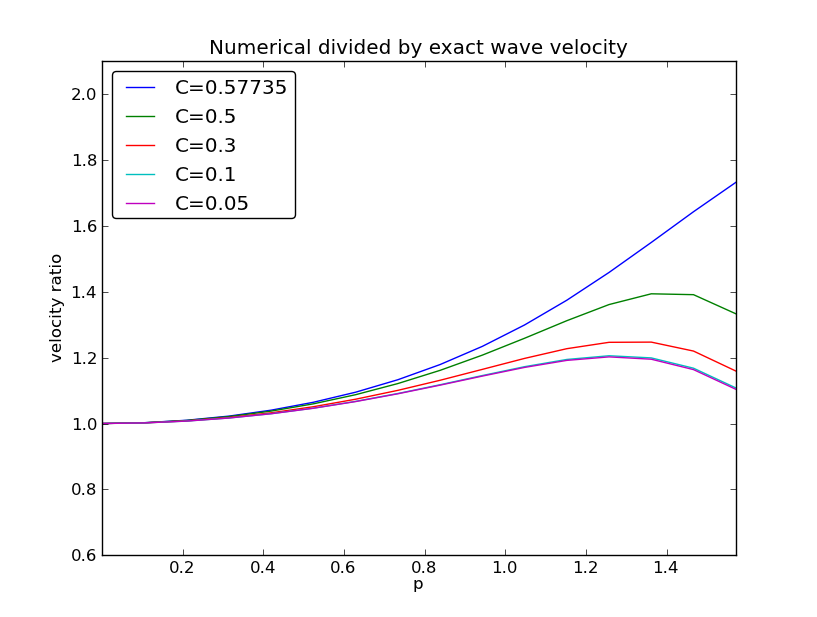
\includegraphics[width=\textwidth]{plot.png}
                \caption{$\tilde{c}/c$ Finite Elements}
                \label{c:plot:fem}
        \end{subfigure}%
        ~ %add desired spacing between images, e. g. ~, \quad, \qquad etc. 
          %(or a blank line to force the subfigure onto a new line)
        \begin{subfigure}[b]{0.55\textwidth}
                \centering
                \includegraphics[width=\textwidth]{disprel.png}
                \caption{$\tilde{c}/c$ Finite Difference}
                \label{c:plot:fd}
        \end{subfigure}
        \caption{Plots comparing the ratio $\tilde{c}/c$ for FEM and FD}\label{c:plots}
\end{figure}

The plot in figure \ref{c:plot:fem} looks a little strange, as we would expect that the ratio is closest to 1 for the value of $C$ that is closest to the stability criterion. In figure \ref{c:plot:fem} however, we see that the ratio is closer to 1 for smaller and smaller $C$.

In comparison, we can look at the corresponding plot that is made from solving \eqref{1D:wave:eq} using finite elements and performing a similar analysis, which is shown in figure \ref{c:plot:fd}. This plot shows the expected behavior.

The plot was generated using the program \texttt{dispersion\_relation.py}, with
\begin{verbatim}
def r(C, p):
    return 1/(C*p)*asin(C*sin(p)/sqrt(1 - 2./3*(sin(p)**2)))  
\end{verbatim}


\subsection{A diagonal M matrix}

It can be very useful to have a diagonal M matrix, as this gives an explicit formula for the coefficients $c_j^n$, so a set of linear equations does not have to be solved at each time level. This decreases the amount of computing significantly.
We can use the trapezoidal rule to produce a diagonal M matrix. Using the program \texttt{fe\_approx\_1D\_numint.py}, and $M\in\mathbb{R}^{5\times5}$, we get the matrix
\begin{equation}
M = \left(\begin{matrix}
\frac{1}{2} h & 0 & 0 & 0 & 0\\
0 & h & 0 & 0 & 0\\
0 & 0 & h & 0 & 0\\
0 & 0 & 0 & h & 0\\
0 & 0 & 0 & 0 & \frac{1}{2} h
\end{matrix}\right)
\end{equation}

We can also find a diagonal matrix by multiplying the matrix M with $e = (1, 1, \hdots, 1)$. This gives a vector with elements that equal the sum of each row from M. In general,

\begin{equation*}
\left[\begin{matrix}
a_{0,0} & a_{0,1} & a_{0,2}\\
a_{1,0} & a_{1,1} & a_{1,2}\\
a_{2,0} & a_{2,1} & a_{2,2}
\end{matrix}\right]
\left[\begin{matrix}
1 \\
1 \\
1
\end{matrix}\right]
 = 
 \left[\begin{matrix}
a_{0,0} + a_{0,1} + a_{0,2} \\
a_{1,0} + a_{1,1} + a_{1,2}\\
a_{2,0} + a_{2,1} + a_{2,2}
\label{def:m:by:ones}
\end{matrix}\right]
\end{equation*}

We then use the matrix created by $diag(w)$, which is the matrix with the elements of $w$ on the diagonal. For $M\in\mathbb{R}^{5\times5}$, we get the matrix

\begin{equation*}
Me =\frac{h}{6}\left[\begin{matrix}
2 & 1 & 0 & 0 & 0\\
1 & 4 & 1 & 0 & 0\\
0 & 1 & 4 & 1 & 0\\
0 & 0 & 1 & 4 & 1\\
0 & 0 & 0 & 1 & 2
\end{matrix}\right]
\left[\begin{matrix}
1 \\
1 \\
1
\end{matrix}\right]
= 
\left[\begin{matrix}
\frac{h}{6}(2 + 1) \\
\frac{h}{6}(1 + 4 + 1) \\
\frac{h}{6}(1 + 4 + 1) \\
\frac{h}{6}(1 + 4 + 1) \\
\frac{h}{6}(2 + 1)
\end{matrix}\right]
=
\left[\begin{matrix}
\frac{1}{2}h \\
h \\
h \\
h \\
\frac{1}{2}h
\end{matrix}\right]
\end{equation*}

\begin{equation*}
diag(Me) =\left[\begin{matrix}
\frac{1}{2} h & 0 & 0 & 0 & 0\\
0 & h & 0 & 0 & 0\\
0 & 0 & h & 0 & 0\\
0 & 0 & 0 & h & 0\\
0 & 0 & 0 & 0 & \frac{1}{2} h
\end{matrix}\right]
\end{equation*}

We see that this gives the same result as using the trapezoidal method. By definition (see \eqref{def:m:by:ones},  this is also the same as replacing each row in the element matrices associated with M by the row sum on the diagonal.



\end{document}